\documentclass{article}

\usepackage{tikz}%调用宏包tikz
\usepackage{circuitikz}%调用宏包circuitikz

\begin{document}

\begin{figure}[h!]%使用figure环境
  \begin{center}
    \begin{circuitikz}
      \draw (0,0)%坐标(0,0)做为起始点,(0,2)做为终点,绘制电压源。_V_代表电压源,_v=$U_q$_绘制标识。
      to[V,v=$U_q$] (0,2) % 电压源
      to[short] (2,2)%坐标(2,2)做为起始点,(2,0)做为终点,绘制电阻。_R_代表电压源,_R=$R_1$_绘制标识。
      to[R=$R_1$] (2,0) % 电阻
      to[short] (0,0);%注意结尾的分号!
    \end{circuitikz}
    \caption{first circuit.}%添加标题
  \end{center}
\end{figure}

\begin{figure}[h!]
  \begin{center}
    \begin{circuitikz}
      \draw (0,2)%坐标(0,2)做为起始点,(0,0)做为终点,绘制电压源。_V_代表电压源,_v=$U_q$_绘制标识。
      to[V,v=$U_q$] (0,0) %(0,0)为终点。
      to[short] (2,0)%由点(0,0)短接至点(2,0)
      to[R=$R_1$] (2,2) %坐标(2,0)做为起始点,(2,2)做为终点,绘制电阻。_R_代表电压源,_R=$R_1$_绘制标识。
      to[short] (0,2);%由点(2,2)短接至点(0,2).注意结尾的分号!
    \end{circuitikz}
    \caption{second circuit.}
  \end{center}
\end{figure}

\begin{figure}[h!]
  \begin{center}
    \begin{circuitikz}
      \draw (0,0)
      to[V,v=$U_q$] (0,2)   % 电压源
      to[short] (2,2)
      to[R=$R_1$] (2,0)    % 电阻
      to[short] (0,0);
      \draw (2,2)
      to[short] (4,2)
      to[L=$L_1$] (4,0)   % 电感
      to[short] (2,0);
     \end{circuitikz}
    \caption{third circuit.}
  \end{center}
\end{figure}

\begin{figure}[h!]
  \begin{center}
    \begin{circuitikz}
      \draw (0,0)
      to[V,v=$U_q$] (0,2) % 电压源
      to[short] (2,2)
      to[R=$R_1$] (2,0) % 电阻
      to[short] (0,0);
      \draw (2,2)
      to[short] (4,2)
      to[L=$L_1$] (4,0)  % 电感
      to[short] (2,0);
      \draw (4,2)
      to[short] (6,2)
      to[C=$C_1$] (6,0)  % 电容
      to[short] (4,0);
    \end{circuitikz}
    \caption{fourth circuit.}
  \end{center}
\end{figure}

\begin{figure}[h!]
	\begin{center}
		\begin{circuitikz}
			  \draw (0,0) node[npn](npn1) {}
			  (npn1.base) node[anchor=east] {B}
			  (npn1.collector) node[anchor=south] {C}
			  (npn1.emitter) node[anchor=north] {E};
		\end{circuitikz}
 		\caption{fifth circuit.}
  	\end{center}
\end{figure}

\begin{figure}[h!]
  \begin{center}
    \begin{circuitikz}
      \draw (0,0)
      to[V,v=$U_q$,i<^=$i_q$] (0,2) % 电压源
      to[short] (2,2)
      to[R=$R_1$,i^<=$i_R$] (2,0) % 电阻
      to[short,*-] (0,0);
      \draw (2,2)
      to[short,*-] (4,2)
      to[L=$L_1$,i^<=$i_L$] (4,0)  % 电感
      to[short,*-]  (2,0);
      \draw (4,2)
      to[short,*-] (6,2)
      to[C=$C_1$,i^<=$i_C$] (6,0)  % 电容
      to[short] (4,0);
      \draw (4,0) to[short] node[ground] {GND} (4,-0.5);
    \end{circuitikz}
    \caption{sixth circuit.}
  \end{center}
\end{figure}

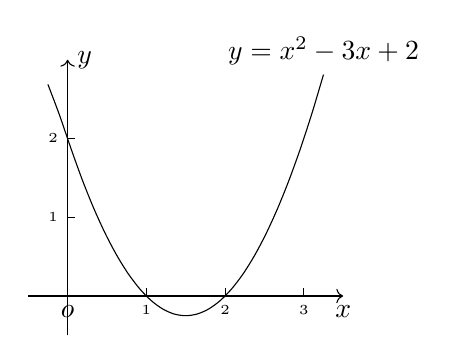
\begin{tikzpicture}
\draw[->](-0.5,0)--(3.5,0) node[below] {$x$};
%绘制(draw)x轴,线到箭头(->),从(-0.5,0)到(3.5,0),文字($x$)显示在线下方(below)
\draw[->](0,-0.5)--(0,3) node[right] {$y$};
%绘制(draw)y轴,线到箭头(->),从(-0.5,0)到(3.5,0),文字($y$)显示在线右侧(below)
\draw plot[smooth, domain = -0.25:3.25] (\x,{\x^2 - 3*\x + 2}) node[above] {$y = x^2 - 3x + 2$};
%绘制(draw)x(\x)到y = x^2 - 3x + 2({\x^2 - 3*\x + 2})的映射,平滑化(smooth),x取值范围为(-0.25,3.25),文字($y = x^2 - 3x + 2$)显示在图像上方(above)
\foreach \x in {1,2,3} {\draw(\x,0)--(\x,0.1) node[below, font = \tiny] at(\x,0) {\x};}
%x轴上的点:(1,0)、(2,0)、(3,0)(\foreach \x in {1,2,3}),在其位置(at(\x,0))绘制(draw)从(x,0)到(x,0.1),字体(font = \tiny),文字(\x)显示在下方(below)
\foreach \y in {1,2} {\draw(0,\y)--(0.1,\y) node[left, font=\tiny] at(0,\y) {\y};}
%y轴上的点:(0,1)、(0,2)(\foreach \y in {1,2}),在其位置(at(0,\y))绘制(draw)从(0,y)到(0.1,y),字体(font = \tiny),文字(\y)显示在下方(below)
\draw(0,0) node[below] {$o$};
%在(0,0)处绘制(draw)零点,字体($o$)显示在下方(below)
\end{tikzpicture}

\end{document}